%%%%%%%%%%%%%%%%%%%%%%%%%%%%%%%%%%%%%%%%%%%%%%%%%%%%%%%%%%%%%%%%%%%%%%%%%%%%%%%%%%%%%%%
%%%%%%%%%%%%%%%%%%%%%%%%%%%%%%%%%%%%%%%%%%%%%%%%%%%%%%%%%%%%%%%%%%%%%%%%%%%%%%%%%%%%%%%
%%%%%%%%%%%%%%%%%%%%%%%%%%%%%%%%%%%%%%%%%%%%%%%%%%%%%%%%%%%%%%%%%%%%%%%%%%%%%%%%%%%%%%%
\section{ Mapeamento com uma função $h_{\VECTOR{c}}(\VECTOR{x}):~\mathbb{R}^N \rightarrow \mathbb{R}$}
\index{Problema inverso: Aplicado!Não linear}
\index{Regressão não linear!Múltipla!Função $h_{\VECTOR{c}}(\VECTOR{x}):~\mathbb{R}^N \rightarrow \mathbb{R}$}
\index{Mapeamento!Função $h_{\VECTOR{c}}(\VECTOR{x}):~\mathbb{R}^N \rightarrow \mathbb{R}$}


\begin{theorem}[Mapeamento usando um polinômio 
$h_{\VECTOR{c}}(\VECTOR{x})$:]
\label{theo:maphcxrnr1}
~\\
\begin{minipage}{0.4\textwidth}
\centering
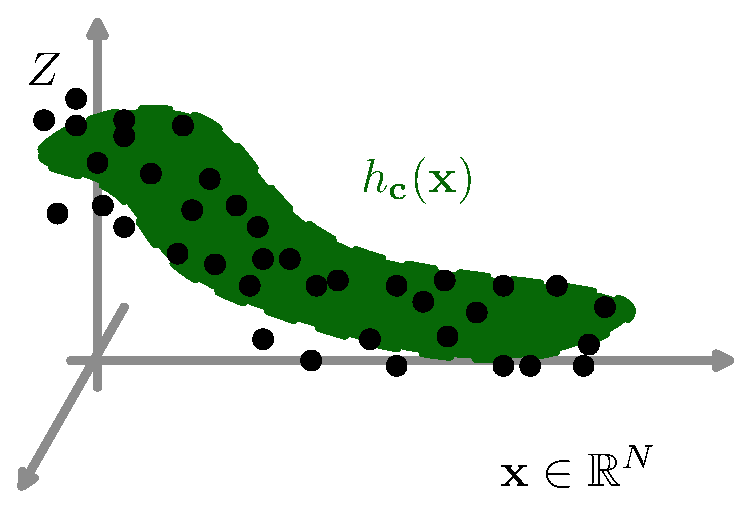
\includegraphics[width=0.95\linewidth]{chapters/mapeamento/mapeamento-hxn-nonlinear.eps} 
\end{minipage}
\begin{minipage}{0.6\textwidth}
Dados,
o escalar $z \in \mathbb{R}$, os vetores coluna  $\VECTOR{x} \in \mathbb{R}^N$ e $\VECTOR{c} \in \mathbb{R}^M$, e 
definida a Eq. (\ref{eq:maphcxrnr1:1}), 
\begin{equation}\label{eq:maphcxrnr1:1}
z=h_{\VECTOR{c}}(\VECTOR{x})\equiv h(\VECTOR{c},\VECTOR{x}),
\end{equation}
onde $h_{\VECTOR{c}}:\mathbb{R}^N \rightarrow \mathbb{R}$, 
é uma função com dominio em $\mathbb{R}^N$ com pontos $\VECTOR{x}$, contradominio em $Z$
e com coeficientes $c_m$ que formam o vetor $\VECTOR{c}$;
podemos afirmar que o vetor $\VECTOR{c}=\VECTOR{\hat{c}}$,
que minimiza o erro $e(\VECTOR{c})$,
\end{minipage}

\begin{equation}\label{eq:maphcxrnr1:2}
e(\VECTOR{c}) =  ||\VECTOR{h}(\VECTOR{c})-\VECTOR{z}||_{\MATRIX{W}}^2 + \alpha||\VECTOR{c}-\VECTOR{c}_{last}||_{\MATRIX{D}}^2,
\end{equation}
onde $\alpha \in \mathbb{R}_+$ é um multiplicador de Lagrange escolhido por nós,
\begin{equation}
\VECTOR{h}(\VECTOR{c})\equiv \VECTOR{h}_{\VECTOR{x}}(\VECTOR{c})=\begin{bmatrix}
h(\VECTOR{c},\VECTOR{x}_1)\\ 
h(\VECTOR{c},\VECTOR{x}_2)\\ 
%\vdots\\ 
%h(\VECTOR{c},\VECTOR{x}_n)\\ 
\vdots\\ 
h(\VECTOR{c},\VECTOR{x}_N)
\end{bmatrix},
~
%\MATRIX{P}=\begin{bmatrix}
%\VECTOR{x}_1^{\transpose}\\ 
%\VECTOR{x}_2^{\transpose}\\ 
%%\vdots\\ 
%%\VECTOR{x}_n^{\transpose}\\ 
%\vdots\\ 
%\VECTOR{x}_N^{\transpose}
%\end{bmatrix},
%~
\VECTOR{z}=\begin{bmatrix}
z_1\\ 
z_2\\ 
%\vdots\\ 
%z_n\\ 
\vdots\\ 
z_N
\end{bmatrix},
~
\MATRIX{W}=\funcdiag\left(\begin{bmatrix}
w_1\\ 
w_2\\ 
%\vdots\\ 
%w_n\\ 
\vdots\\ 
w_N
\end{bmatrix}\right),
~
\MATRIX{D}=\funcdiag\left(\begin{bmatrix}
d_1\\ 
d_2\\ 
%\vdots\\ 
%d_m\\ 
\vdots\\ 
d_M
\end{bmatrix}\right);
\end{equation}
pode ser achado\footnote{A demostração pode ser vista na Prova \ref{proof:theo:maphcxrnr1}.} 
usando de forma iterativa a Eq. (\ref{eq:maphcxrnr1:3})
\begin{equation}\label{eq:maphcxrnr1:3}
\VECTOR{c}_{i}=\VECTOR{c}_{i-1}-[\MATRIX{J}(\VECTOR{c}_{i-1})^{\transpose}\MATRIX{W}\MATRIX{J}(\VECTOR{c}_{i-1})+\alpha \MATRIX{D}]^{-1}\MATRIX{J}(\VECTOR{c}_{i-1})^{\transpose}\MATRIX{W}[\VECTOR{h}(\VECTOR{c}_{i-1})-\VECTOR{z}],
\end{equation}
onde a matriz $\MATRIX{J}(\VECTOR{c})$ 
$\equiv \frac{\partial \VECTOR{h}(\VECTOR{c})}{\partial \VECTOR{c}^{\transpose}}$ é a 
\hyperref[def:jacobian]{\textbf{matriz Jacobiana}}  de $\VECTOR{h}(\VECTOR{c})$,
\begin{equation}
\MATRIX{J}(\VECTOR{c})\equiv \MATRIX{J}_{\VECTOR{c}}(\VECTOR{c})=\begin{bmatrix}
\VECTOR{j}(\VECTOR{c},\VECTOR{x}_1)\\ 
\VECTOR{j}(\VECTOR{c},\VECTOR{x}_2)\\ 
%\vdots\\ 
%\VECTOR{j}(\VECTOR{c},\VECTOR{x}_n)\\ 
\vdots\\ 
\VECTOR{j}(\VECTOR{c},\VECTOR{x}_N)
\end{bmatrix},
\quad
\begin{array}{lll}
\VECTOR{j}(\VECTOR{c},\VECTOR{x}) & = & \frac{\partial h(\VECTOR{c},\VECTOR{x})}{\partial \VECTOR{c}^{\transpose}} \\
                       ~ & ~ & ~\\
                       ~ & = & \left[\frac{\partial h(\VECTOR{c},\VECTOR{x})}{\partial c_1}\quad \frac{\partial h(\VECTOR{c},\VECTOR{x})}{\partial c_2}\quad ...\quad \frac{\partial h(\VECTOR{c},\VECTOR{x})}{\partial c_{m}} \quad ... \quad \frac{\partial h(\VECTOR{c},\VECTOR{x})}{\partial c_{M}} \right]
\end{array}
\end{equation}

\textbf{Considerações:}
\begin{itemize}
\item A busca iterativa da Eq. (\ref{eq:maphcxrnr1:3}) 
é declarada finalizada com sucesso 
quando iterações consecutivas do vetor $\VECTOR{c}_i$ convergem a valores próximos, onde declaramos $\VECTOR{\hat{c}}=\VECTOR{c}_i$.
\item O erro mínimo, $e(\VECTOR{\hat{c}}) \geq 0$, não necessariamente ter valor zero. 
\end{itemize}
\end{theorem}

%\begin{tcbattention}
%\begin{itemize}
%\item 
%\end{itemize}
%\end{tcbattention}

%%%%%%%%%%%%%%%%%%%%%%%%%%%%%%%%%%%%%%%%%%%%%%%%%%%%%%%%%%%%%%%%%%%%%%%%%%%%%%%%
\subsection{Exemplos de mapeamento usando uma função
$h_{\VECTOR{c}}(\VECTOR{x}):~\mathbb{R}^N \rightarrow \mathbb{R}$}

\begin{example}\label{ex:theo:maphcxrnr1}
Conhecida as $N=16$ amostras $\VECTOR{x}_n$ e $z_n$, mostradas nas  Tabelas \ref{table:theo:maphcxrnr1:xn} e \ref{table:theo:maphcxrnr1:zn},
achar os parametros $c_m$ do vetor $\VECTOR{c}=[c_1\quad c_2\quad c_3]^{\transpose}$ da função $h(\VECTOR{c},x)$, 
\begin{equation}
h(\VECTOR{c},\VECTOR{x})=c_1 e^{-\left(\frac{x_1}{c_2}\right)^{-4}-\left(\frac{x_2}{c_2}\right)^{-4}}+c_3,
\end{equation}
que gere o menor erro 
$e(\VECTOR{c})=\sum_{n=1}^{N} ||h(\VECTOR{c},\VECTOR{x}_n)-z_n||^2 + 0.1 ||\VECTOR{c}-\VECTOR{c}_{last}||^2$.
\end{example}


\begin{table}[h!]
\centering
\begin{tabular}{|c|c|c|c|c|c|c|c|c|} 
 \hline
$n$   & 1 & 2 & 3 & 4 & 5 & 6 & 7 & 8\\ \hline
$\VECTOR{x}_n$ & 5.24910 & 5.28851 & 5.58188 & 2.25455 & 0.17769 & 3.65716 & 5.00074 & 2.37936 \\ 
             ~ & 5.80108 & 2.29459 & 2.94123 & 4.97383 & 4.84170 & 3.20595 & 2.36837 & 1.46028 \\ \hline
 \hline
$n$   & 9 & 10 & 11 & 12 & 13 & 14 & 15 & 16\\  \hline
$\VECTOR{x}_n$ & 1.13752 & 5.49762 & 4.08773 & 1.90381 & 0.06277 & 0.98381 & 3.67799 & 2.21287 \\
             ~ & 0.01718 & 3.69885 & 5.13457 & 5.56777 & 4.26294 & 3.95342 & 5.68502 & 1.08792 \\ \hline
\end{tabular}
\caption{Valores $\VECTOR{x}_n$.}
\label{table:theo:maphcxrnr1:xn}
\end{table}

\begin{table}[h!]
\centering
\begin{tabular}{|c|c|c|c|c|c|c|c|c|} 
 \hline
$n$   & 1 & 2 & 3 & 4 & 5 & 6 & 7 & 8\\ \hline
$y_n$ & 1.9005 & 2.1166 & 2.0181 & 1.9069 & 2.1991 & 2.4291 & 1.8024 & 7.0944  \\ \hline
 \hline
$n$   & 9 & 10 & 11 & 12 & 13 & 14 & 15 & 16\\  \hline
$y_n$ & 9.6170 & 2.1098 & 1.9972 & 1.8631 & 2.3673 & 2.2807 & 2.0231 & 8.0547 \\ \hline
\end{tabular}
\caption{Valores $y_n$.}
\label{table:theo:maphcxrnr1:zn}
\end{table}

\begin{SolutionT}[Relativa ao Exemplo \ref{ex:theo:maphcxrnr1}:]\label{sol:theo:maphcxrnr1}
Para obter  o vetor $\VECTOR{c}=\VECTOR{\hat{c}}$
que provoque o menor erro $e(\VECTOR{c})$,
podemos usar iterativamente a Eq. (\ref{eq:maphcxrnr1:3}), com 
\begin{equation}
\frac{\partial h(\VECTOR{c},\VECTOR{x})}{\partial c_1} 
= e^{-\left(\frac{x_1}{c_2}\right)^{-4}-\left(\frac{x_2}{c_2}\right)^{-4}},\qquad 
\frac{\partial h(\VECTOR{c},\VECTOR{x})}{\partial c_2} 
= 4\frac{c_1}{c_2}\left(\left(\frac{x_1}{c_2}\right)^{-4}+\left(\frac{x_2}{c_2}\right)^{-4}\right)e^{-\left(\frac{x_1}{c_2}\right)^{-4}-\left(\frac{x_2}{c_2}\right)^{-4}}, 
\end{equation} 
$\frac{\partial h(\VECTOR{c},\VECTOR{x})}{\partial c_3} =1$,
iniciando em $\VECTOR{c}_{0}=[3\quad 2\quad 1]^{\transpose}$ escolhido arbitrariamente.
Obtendo assim a Tabela \ref{table:theo:maphcxrnr1:ei}, que conclui em
$\VECTOR{\hat{c}}=\VECTOR{c}_{5}=[7.8170\quad 3.0761\quad 1.9981]^{\transpose}$,
com  um erro $e(\VECTOR{c}_{5})=0.27067$.


\begin{table}[h!]
\centering
\begin{tabular}{|c|c|c|c|c|c|c|} 
 \hline
$i$   & 0 & 1 & 2 & 3 & 4 & 5 \\ \hline
\hline
$c_1$ & 3.0000 & 6.2450 & 5.2762 & 7.5557 & 7.7751 & 7.8170 \\ \hline
$c_2$ & 2.0000 & 4.6303 & 2.9364 & 3.1952 & 3.0813 & 3.0761 \\ \hline
$c_3$ & 1.0000 & 2.1159 & 3.3712 & 2.0283 & 2.0026 & 1.9981 \\ \hline
\hline
$e(\VECTOR{c}_{i})$ & 125.55885 & 45.42202 & 25.33905 & 0.47703 & 0.27315 & 0.27067  \\ \hline
\end{tabular}
\caption{Valores $e(\VECTOR{c}_{i})$ e vetores $\VECTOR{c}_{i}$.}
\label{table:theo:maphcxrnr1:ei}
\end{table}

    \begin{figure}[!h]
        \centering
        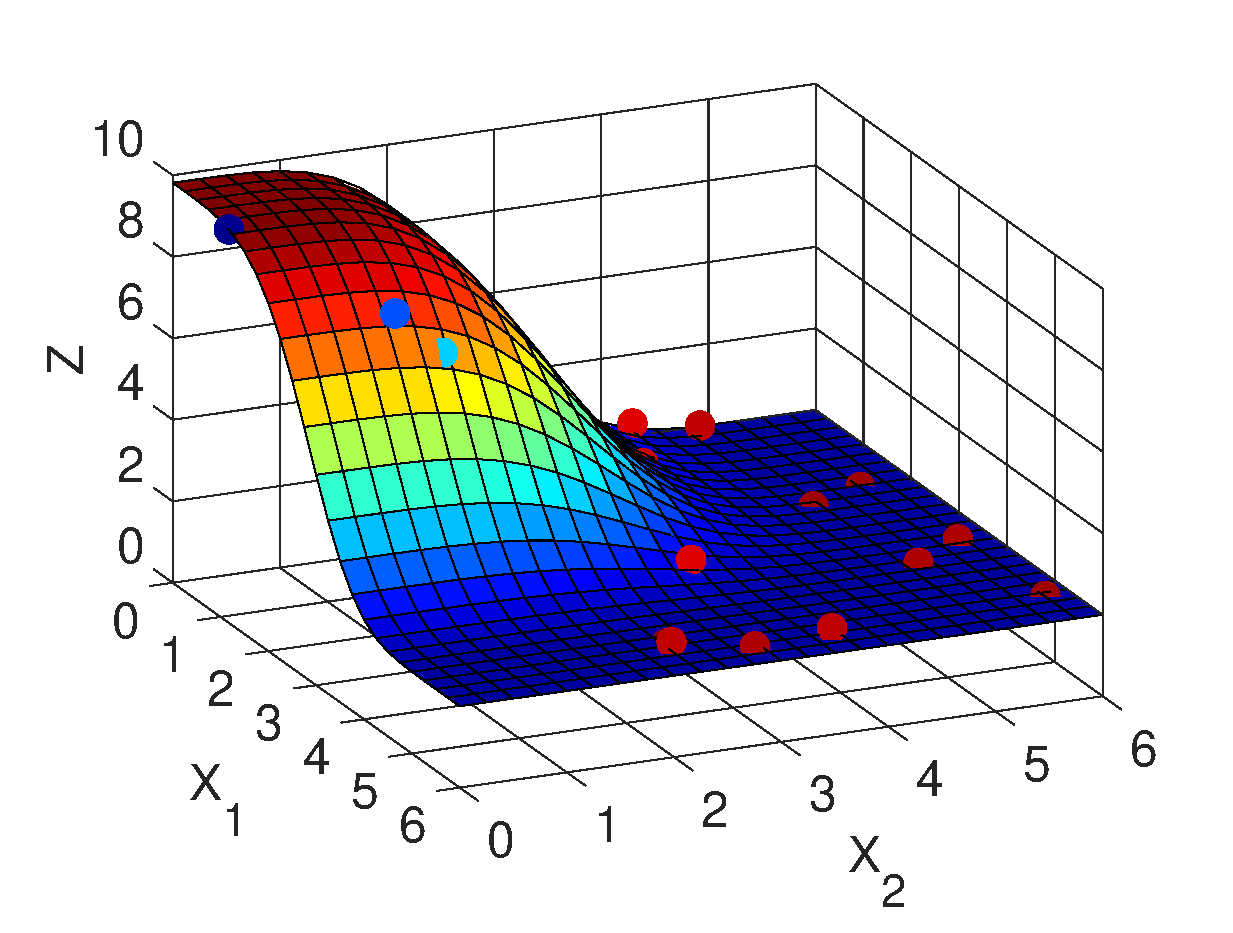
\includegraphics[width=0.49\textwidth]{chapters/mapeamento/mfiles/mapeamentornr1-nonlinear/minimizando_hx.eps}
        \caption{Gráfico das amostras $\{\VECTOR{x}_n,z_n\}$ e da superfície $\VECTOR{x}$ vs. $h(\VECTOR{c}_5,\VECTOR{x})$.}
        \label{fig:theo:maphcxrnr1:xnyn}
    \end{figure}

\end{SolutionT}


